% This is the master file of the folder structure. In order to compile your document, run this file. In most LaTeX editors, the master file can be specified such that the document can also be compiled from the other .tex files (in the docs folder).

% First, the preamble needs to be called. This contains all the 'under the hood' stuff for your document.
% This file contains your LaTeX preamble. A preamble is a part of your document where all required packages and macros can be defined. This needs to be done before the \begin{document} command.

% Documentclass:
% Standard LaTeX classes are: article, book, report, slides, and letter. These cover the basis, but are not best. More advanced users might want to try out the KOMA classes or the memoir class. Optional arguments: 10pt. The font size of the main content is set to 10pt with the option between [].
\documentclass[10pt]{report}
 \usepackage[dutch]{babel}
% Geometry:
% The papersize of the document is defined with the geometry package. Here, the size is set to A4 with a4paper. Other possibilities are a5paper, b5paper, letterpaper, legalpaper and executivepaper.
\usepackage[a4paper]{geometry}

% AMS math packages:
% Required for proper math display.
\usepackage{amsmath,amsfonts,amsthm}

% Graphicx:
% If you want to include graphics in your document, the graphicx package is required.
\usepackage{graphicx}

% Booktabs:
% The booktabs package is needed for better looking tables. 
\usepackage{booktabs}

% SIunitx:
% The SIunitx package enables the \SI{}{} command. It provides an easy way of working with (SI) units.
\usepackage{siunitx}

% URL:
% Clickable URL's can be made with this package: \url{}.
\usepackage{url}

% Caption:
% For better looking captions. See caption documentation on how to change the format of the captions.
\usepackage{caption}

% Hyperref:
% This package makes all references within your document clickable. By default, these references will become boxed and colored. This is turned back to normal with the \hypersetup command below.
\usepackage{hyperref}
	\hypersetup{colorlinks=false,pdfborder=0 0 0}

% Cleveref:
% This package automatically detects the type of reference (equation, table, etc.) when the \cref{} command is used. It then adds a word in front of the reference, i.e. Fig. in front of a reference to a figure. With the \crefname{}{}{} command, these words may be changed.
\usepackage{cleveref}
	\crefname{equation}{equation}{equations}
	\crefname{figure}{figure}{figures}	
	\crefname{table}{table}{tables}
\newcommand{\projectname}{PROJECT}
\newcommand{\projectname}{PROJECT}

% The title page is created with the command \maketitle which needs to be placed after the \begin{document} command. To create the titlepage, some entries are needed: the name of the autor is defined by \author{}, the title by the entry \title{} and the date by the command \date{}. Note that the current date is displayed with \today.
\author{Johannes Michel\\Robbert van Nijnatten\\Raymond Rohder\\Vincent Stout\\Kevin van der Vleuten}
\title{Plan van aanpak - \projectname}
\date{\today}

% All the actual content of your document should be placed after \begin{document} and before \end{document}. This content should be placed in the docs folder and can then be called with \input{docs/filename}.
\begin{document}

% Here the actual title page is printed, based on the given entries \author{}, \title{} and \date{}.
\maketitle

% The table of contents can be automatically generated with the \tableofcontents command. Note that you need to compile the document twice in order to see the changes in the table of contents.
\renewcommand*\contentsname{Inhoud}
\tableofcontents

% The \input{} command reads and processes the indicated example.tex file. Note that docs/ locates the folder where the .tex file is stored.
%% A chapter named 'Your first document' is created
\chapter{Your first document} \label{cha:your-first-document}


% A section called 'Basics' is created
\section{Basics} \label{sec:basics}

Text is formatted with: \textbf{bold}, \textit{italic} and \underline{underline}.
\Cref{sec:basics} is part of \cref{cha:your-first-document}.


% A subsection named 'Typesetting content' is created
\section{Typesetting content} \label{sec:typesetting}


% A subsubsection named 'Equations' is created
\subsection{Equations} \label{subsec:equations}

% Inline equations
An example of an inline equation is: the derivative of $x^2$ is $2x$. \Cref{eq:example} shows a display equation:
% Display equations
\begin{align} \label{eq:example}
          y_{0} &= \frac{\sqrt{256}}{2} \\
                &= 2^{3} = 8 \nonumber 
\end{align}


\subsection{Units} \label{subsec:units}

% % Working with units
An easy way to work with (SI) units: \SI{1}{\hertz} is equal to \SI{2\pi}{\radian\per\second}.


\subsection{Figures} \label{subsec:figures}

% Inserting a figure
Here a figure named \textit{logo.pdf} is inserted\footnote{The \textit{logo.pdf} file is located in the figs folder.}:
\begin{figure}[h]
  \centering
  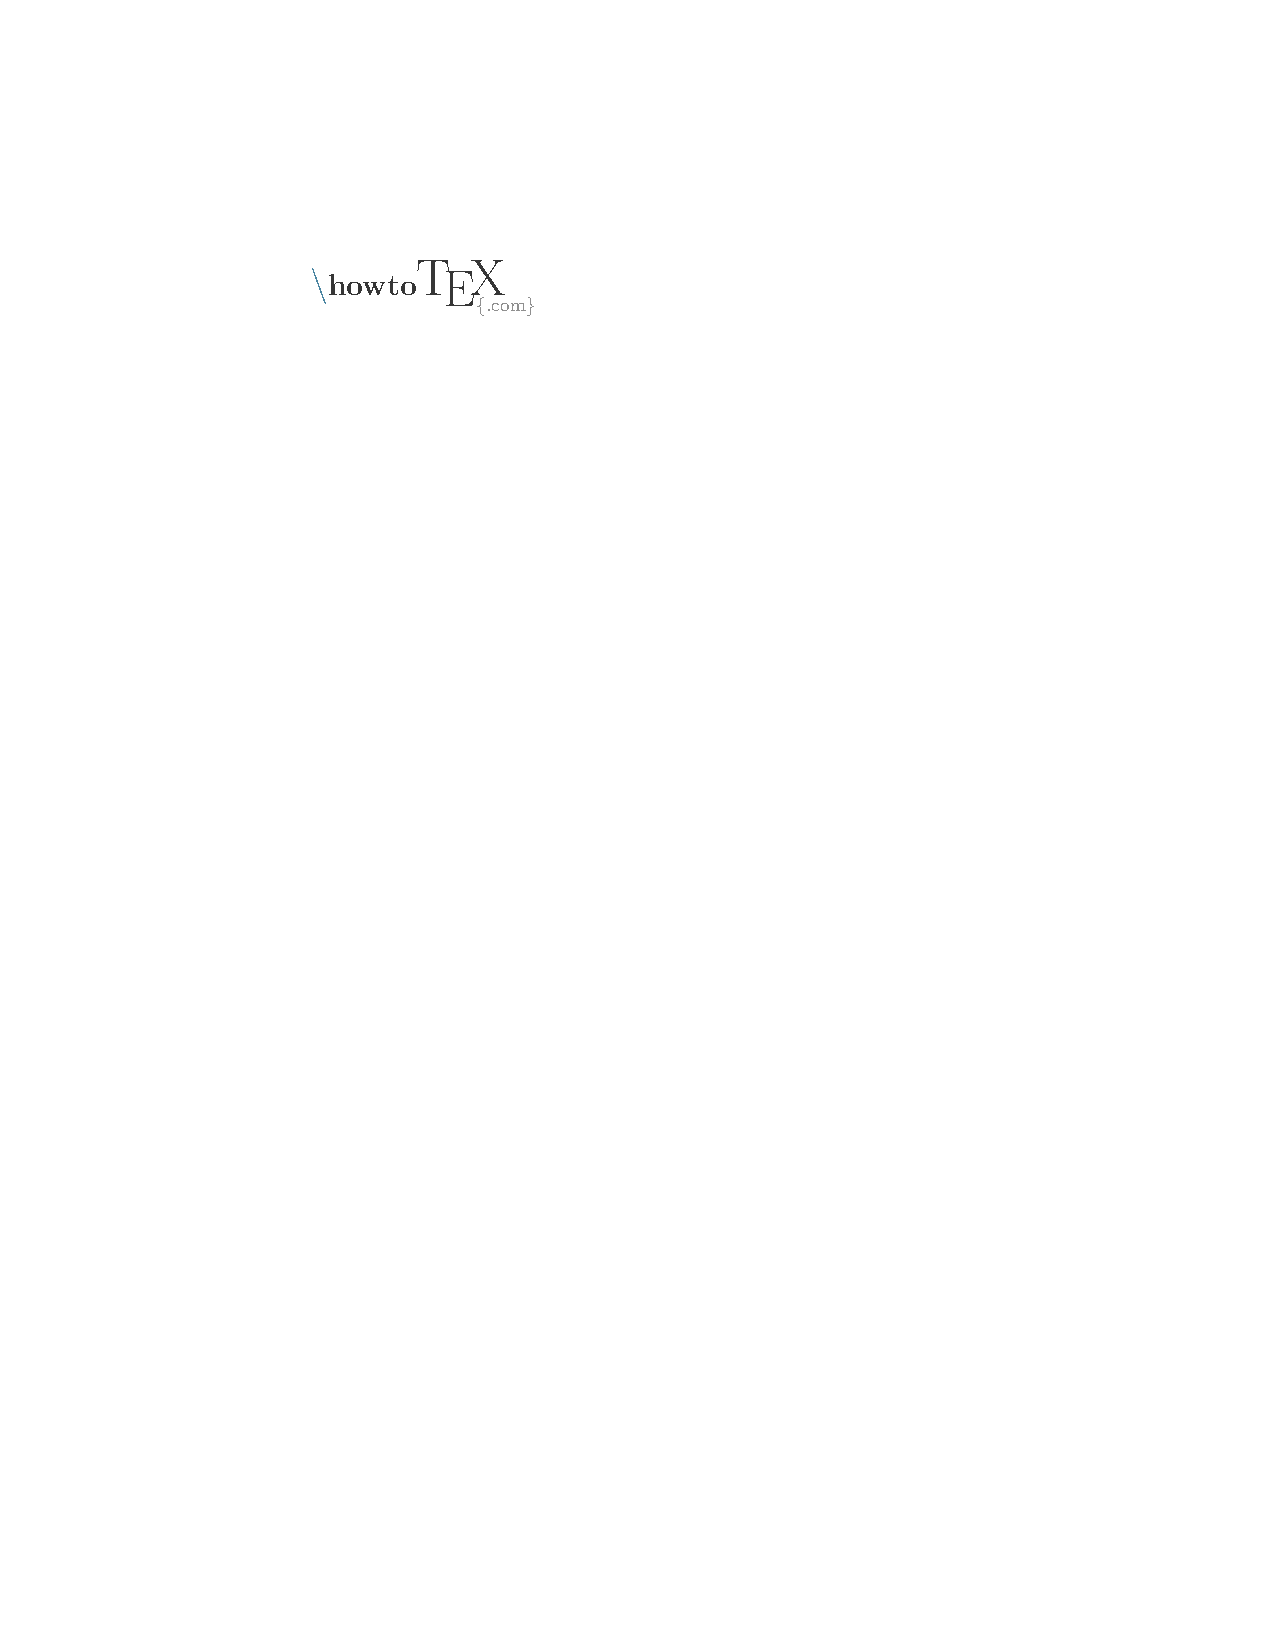
\includegraphics[width=50mm]{figs/logo}
  \caption{Caption example}
  \label{fig:logo}
\end{figure}


\subsection{Tables} \label{subsec:tables}

% Inserting a table
A table is shown in \cref{tb:table}.
\begin{table}[h]
  \centering
  \caption{Caption example}
  \label{tb:table}
  \begin{tabular}{crl}
    \toprule
    Name     & Grade & Year    \\
    \midrule
    John     & 7.5   & 2012\\
    Richard  & 2     & 2010\\
    \bottomrule
  \end{tabular}
\end{table}


\subsection{Lists} \label{subsec:lists}
% Creating lists
%% Here a subsubsection is created. Note that this section is not shown in the table of content.
\subsubsection{Numbered}
Creating a numbered list:
\begin{enumerate}
  \item First entry
  \item Second entry
\end{enumerate}

\subsubsection{Descriptive}
Creating a descriptive list:
\begin{description}
  \item[First] entry
  \item[Second] entry
\end{description}


\section{Reference to bibliography items} \label{sec:bibliography}
First are reference to a website is made \cite{MiscEntry}, then a reference to an article \cite{ArticleEntry} and finally a reference to a book \cite{last2012}.

\paragraph{Good luck!}
% A chapter named 'Your first document' is created

\chapter{Achtergronden} \label{cha:your-first-document}

\section{Opdracht} \label{sec:opdracht}

Dit project is een \underline{augmented reality} project, en maakt gebruik van OpenCV voor motion detection en OpenGL voor de 3D graphics.

Text is formatted with: \textbf{bold}, \textit{italic} and \underline{underline}.
\Cref{sec:basics} is part of \cref{cha:your-first-document}.

\section{Projectnaam} \label{sec:projectnaam}
Het project is genaamd: "\projectname"


\subsection{Opdrachtgever} \label{subsec:opdrachtgever}

% Inline equations
An example of an inline equation is: the derivative of $x^2$ is $2x$. \Cref{eq:example} shows a display equation:
% Display equations
\begin{align} \label{eq:example}
          y_{0} &= \frac{\sqrt{256}}{2} \\
                &= 2^{3} = 8 \nonumber 
\end{align}


\subsection{Units} \label{subsec:units}

% % Working with units
An easy way to work with (SI) units: \SI{1}{\hertz} is equal to \SI{2\pi}{\radian\per\second}.


\subsection{Figures} \label{subsec:figures}

% Inserting a figure
Here a figure named \textit{logo.pdf} is inserted\footnote{The \textit{logo.pdf} file is located in the figs folder.}:
\begin{figure}[h]
  \centering
  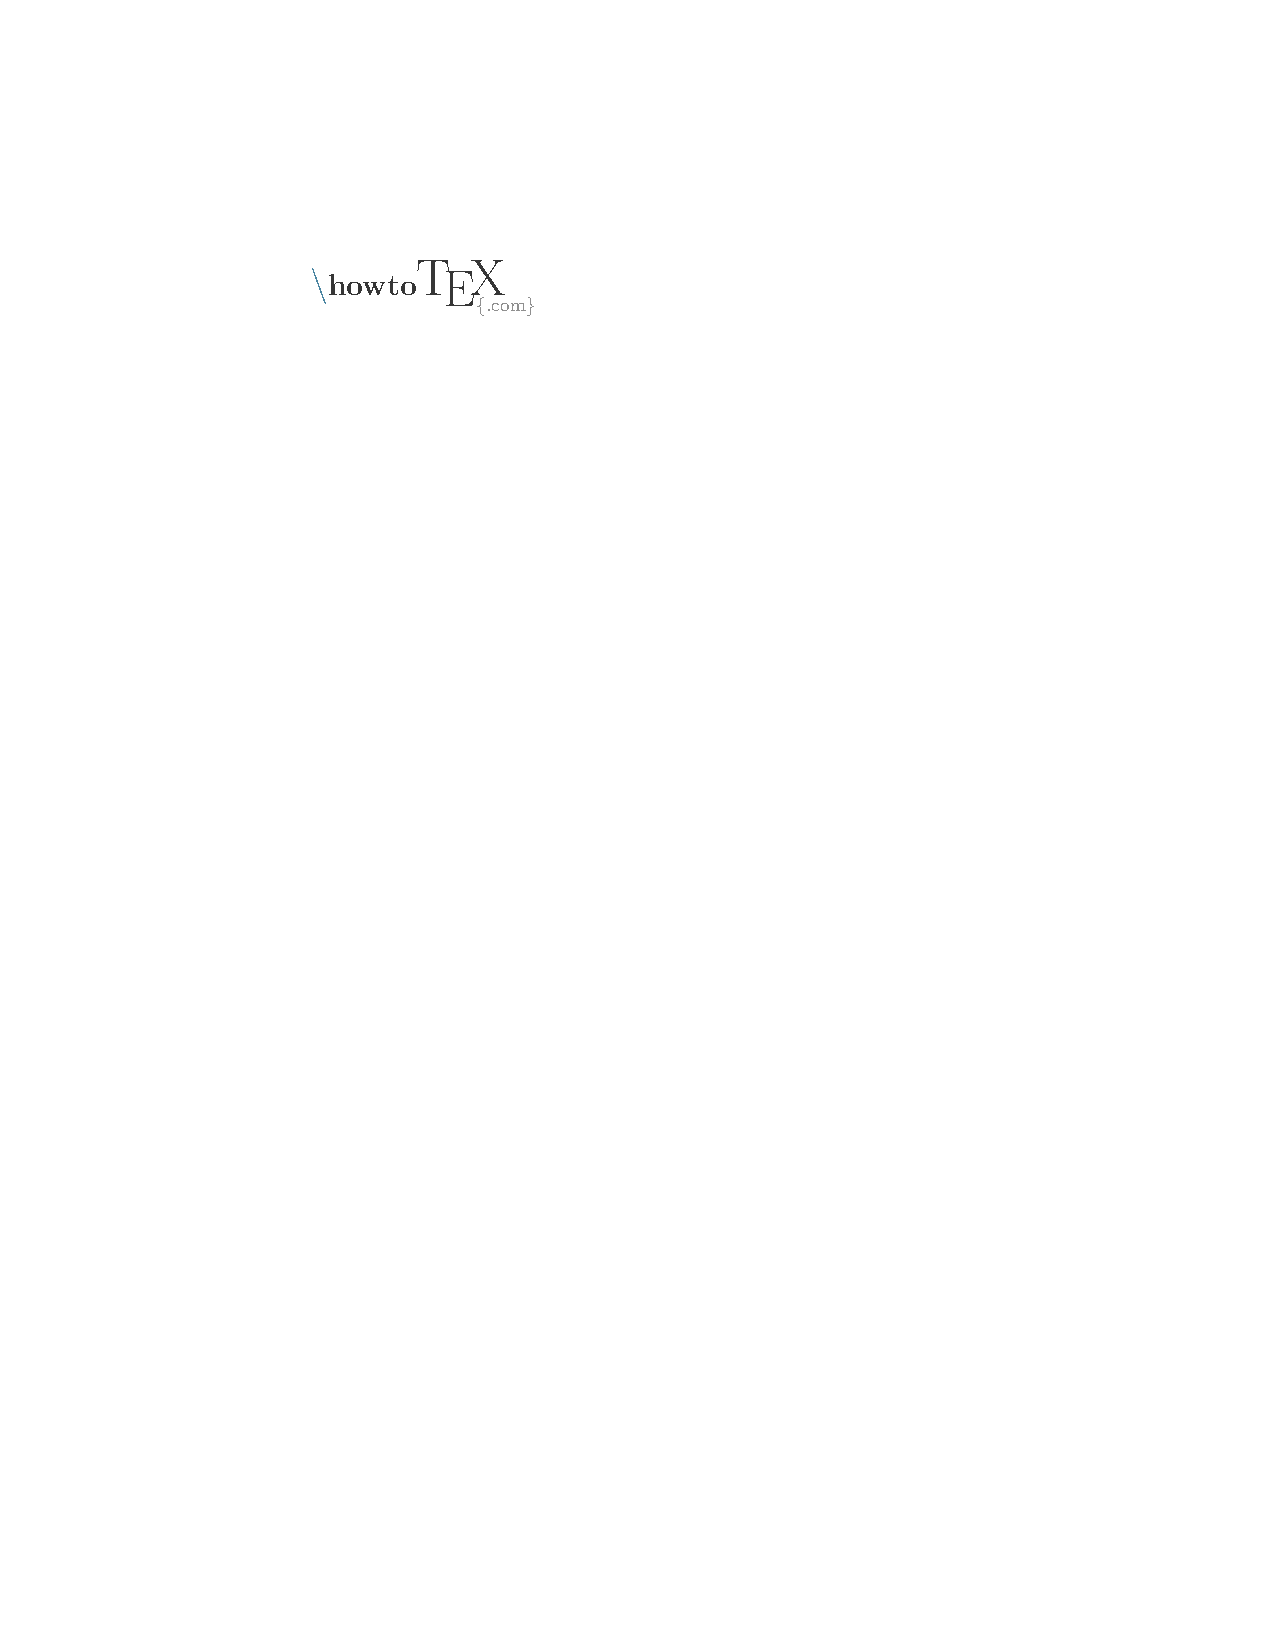
\includegraphics[width=50mm]{figs/logo}
  \caption{Caption example}
  \label{fig:logo}
\end{figure}


\subsection{Tables} \label{subsec:tables}

% Inserting a table
A table is shown in \cref{tb:table}.
\begin{table}[h]
  \centering
  \caption{Caption example}
  \label{tb:table}
  \begin{tabular}{crl}
    \toprule
    Name     & Grade & Year    \\
    \midrule
    John     & 7.5   & 2012\\
    Richard  & 2     & 2010\\
    \bottomrule
  \end{tabular}
\end{table}

\subsection{Lists} \label{subsec:lists}
% Creating lists
%% Here a subsubsection is created. Note that this section is not shown in the table of content.
\subsubsection{Numbered}
Creating a numbered list:
\begin{enumerate}
  \item First entry
  \item Second entry
\end{enumerate}

\subsubsection{Descriptive}
Creating a descriptive list:
\begin{description}
  \item[First] entry
  \item[Second] entry
\end{description}


\section{Reference to bibliography items} \label{sec:bibliography}
First are reference to a website is made \cite{MiscEntry}, then a reference to an article \cite{ArticleEntry} and finally a reference to a book \cite{last2012}.

\paragraph{Good luck!}
\chapter{Projectresultaat} \label{cha:projectresultaat}
Het projectresultaat omschrijft de situatie wanneer PROJECT zijn doel heeft bereikt. Dit aan de hand van een doelstelling en eindvoorwaarden.
\section{Doelstelling} \label{sec:doelstelling}
Het doel van PROJECT is een proof of concept waarbij Augmented Reality centraal staat. De gebruiker komt in aanraking met een met extra informatie aangevulde realiteit.
\section{Eindvoorwaarden} \label{sec:eindvoorwaarden}
\begin{enumerate}
  \item Interactiviteit. Interactie tussen de gebruiker en PROJECT bepaald die inhoud van getoonde informatie.
  \item Computervision. Acties van de gebruiker worden met behulp van een camera vastgelegd en gebruikt als input voor de applicatie.
  \item Informatief. Alle getoonde informatie is dynamisch, contextueel relevant en afgestemd op de gebruiker.
  \item 3D Graphics. De user interface bevat 3D beelden. 
\end{enumerate}
\chapter{Projectactiviteiten} \label{cha:projectactiviteiten}
Ter voorbereiding van dit project zijn hieronder puntsgewijs de te verwachten projectactiviteiten opgesomd.
\section{Vooronderzoek (Sprint 1 - Week 1)} \label{sec:vooronderzoek}
\begin{enumerate}
  \item Brainstormsessie t.b.v. projectopdracht
  \item Resultaat uitwerken tot concept ontwerp
\end{enumerate}
\section{Voorbereiding (Sprint 2 - Week 2)} \label{sec:voorbereiding}
\begin{enumerate}
  \item Opstellen van het Plan van Aanpak en planning
  \item Reviewen en aanpassen van het Plan van Aanpak en planning
  \item Opstellen van het Interaction Design document
  \item Reviewen en aanpassen van het Interaction Design document
\end{enumerate}
\section{Ontwerp (Sprint 3 - Week 3)} \label{sec:ontwerp}
\begin{enumerate}
  \item Opstellen van het Technische ontwerp (klassendiagram)
  \item Reviewen en aanpassen van het Technische ontwerp
\end{enumerate}
\section{Proof of Concept (Sprint 4 - Week 4 en 5)} \label{sec:proofofconcept}
\begin{enumerate}
  \item Uitwerken van het Technische ontwerp tot proof of concept
  \item Onderdelen samenvoegen tot één product
\end{enumerate}
\section{Testen (Sprint 5 - Week 6 en 7)} \label{sec:testen}
\begin{enumerate}
  \item Proof of concept testen op fouten (Debuggen)
  \item Uitwerken van proof of concept tot definitief product
\end{enumerate}
\section{Afronding (Sprint 6 - Week 8)} \label{sec:afronding}
\begin{enumerate}
  \item Opstellen van presentatie en promotie video
  \item Reviewen en aanpassen van de presentatie en promotie video
  \item Definitief product opleveren
\end{enumerate}
\chapter{Projectgrenzen} \label{cha:projectgrenzen}
Om onduidelijkheden te voorkomen dienen de projectvoorwaarden en werkzaamheden afgebakend te worden. Dit pilot-project is een proof of concept en zal niet op de commerciële markt uitgebracht worden.
\\
\begin{enumerate}
  \item PROJECT wordt 'as is' opgeleverd wanneer de opleveringsdatum volgens de planning bereikt is.
  \item PROJECT voorziet de realiteit van extra informatie (Augmented Reality).
  \item PROJECT wordt ontwikkeld voor het Windows-pc platform.
  \item PROJECT maakt gebruik van OpenGL (Open Graphics Library) om 3D-graphics te realiseren.
  \item PROJECT maakt gebruik van OpenCV (Open Source Computer Vision) om real-time computer vision (object herkenning) te realiseren.
\end{enumerate}
% A chapter named 'Your first document' is created
\chapter{Tussenresultaten} \label{cha:your-first-document}


% A section called 'Basics' is created
\section{Basics} \label{sec:basics}

Text is formatted with: \textbf{bold}, \textit{italic} and \underline{underline}.
\Cref{sec:basics} is part of \cref{cha:your-first-document}.


% A subsection named 'Typesetting content' is created
\section{Typesetting content} \label{sec:typesetting}


% A subsubsection named 'Equations' is created
\subsection{Equations} \label{subsec:equations}

% Inline equations
An example of an inline equation is: the derivative of $x^2$ is $2x$. \Cref{eq:example} shows a display equation:
% Display equations
\begin{align} \label{eq:example}
          y_{0} &= \frac{\sqrt{256}}{2} \\
                &= 2^{3} = 8 \nonumber 
\end{align}


\subsection{Units} \label{subsec:units}

% % Working with units
An easy way to work with (SI) units: \SI{1}{\hertz} is equal to \SI{2\pi}{\radian\per\second}.


\subsection{Figures} \label{subsec:figures}

% Inserting a figure
Here a figure named \textit{logo.pdf} is inserted\footnote{The \textit{logo.pdf} file is located in the figs folder.}:
\begin{figure}[h]
  \centering
  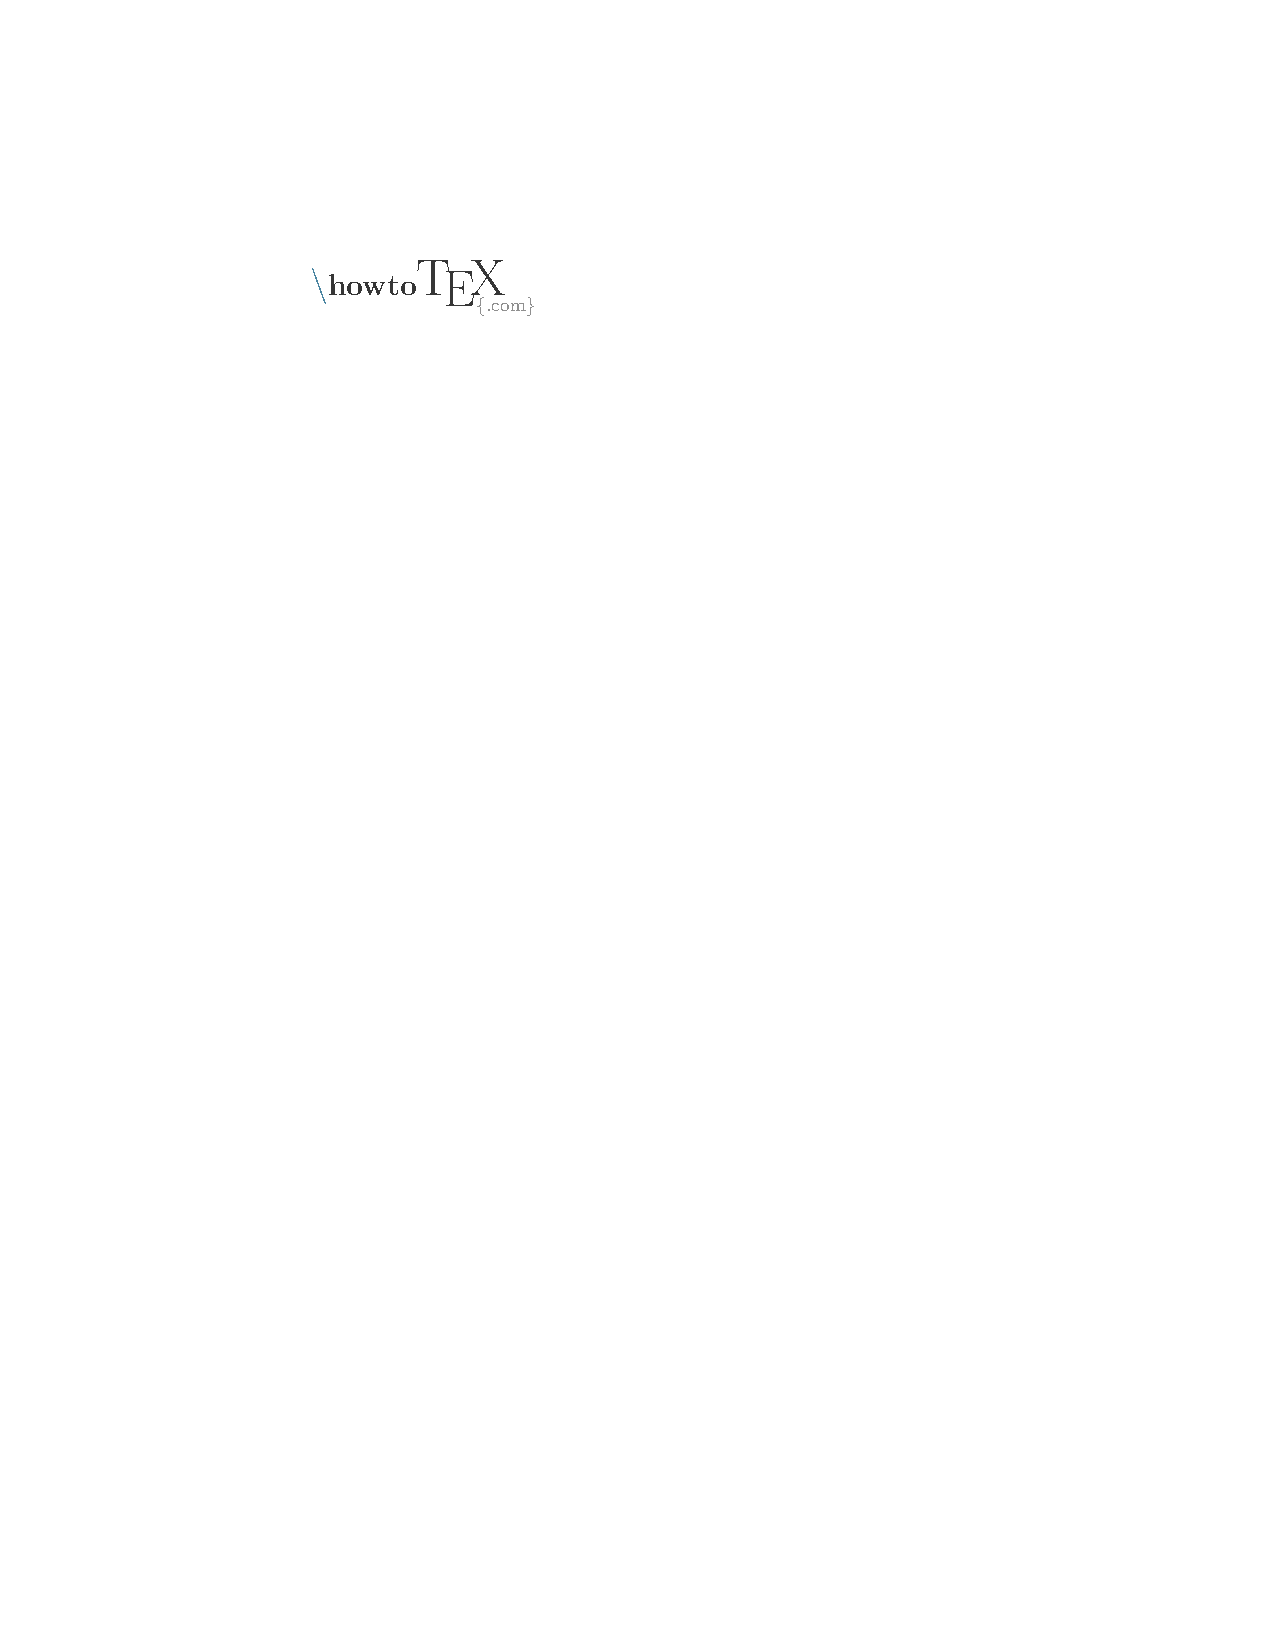
\includegraphics[width=50mm]{figs/logo}
  \caption{Caption example}
  \label{fig:logo}
\end{figure}


\subsection{Tables} \label{subsec:tables}

% Inserting a table
A table is shown in \cref{tb:table}.
\begin{table}[h]
  \centering
  \caption{Caption example}
  \label{tb:table}
  \begin{tabular}{crl}
    \toprule
    Name     & Grade & Year    \\
    \midrule
    John     & 7.5   & 2012\\
    Richard  & 2     & 2010\\
    \bottomrule
  \end{tabular}
\end{table}


\subsection{Lists} \label{subsec:lists}
% Creating lists
%% Here a subsubsection is created. Note that this section is not shown in the table of content.
\subsubsection{Numbered}
Creating a numbered list:
\begin{enumerate}
  \item First entry
  \item Second entry
\end{enumerate}

\subsubsection{Descriptive}
Creating a descriptive list:
\begin{description}
  \item[First] entry
  \item[Second] entry
\end{description}


\section{Reference to bibliography items} \label{sec:bibliography}
First are reference to a website is made \cite{MiscEntry}, then a reference to an article \cite{ArticleEntry} and finally a reference to a book \cite{last2012}.

\paragraph{Good luck!}
\chapter{Kwaliteit} 

\paragraph{Elk project kan in de loop van een traject de oorspronkelijke doelen, waarden en functionaliteiten uit het oog verliezen. Daarom is de kwaliteitbewaking noodzakelijk voor elk project. Hoe dit gebeurt binnen het traject van \projectname\ zal in dit hoofdstuk uitgelegd worden.}
\paragraph{middenstuk, hoe kwaliteitbewaking}
\paragraph{einde, conclusie}

% A chapter named 'Your first document' is created
\chapter{Projectorganisatie} \label{cha:your-first-document}


% A section called 'Basics' is created
\section{Rollen} \label{sec:basics}

\textbf{Projectleiders en projectplanners(Council)}\\
\textbf{naam:}	Raymond Rohder\\
\textbf{email:}	rchrohde@student.avans.nl\\
\\
\textbf{naam:}	Robbert van Nijnatten\\
\textbf{email:}	rvnijnatten@casema.nl\\
\\
De taak van de projectleider is het bewaren van overzicht in het team. Hij is het aanspreekpunt voor alles aangaande het product, en verdeelt de taken binnen het team. De projectleider maakt gebruik van verslagen van de andere projectleden om zijn of haar werk goed te doen. De projectleider rapporteert rechtstreeks aan de senior met de producten en bevindingen van het team.\\
\\
\textbf{Projectsecretaris}\\
\textbf{naam:}	Vincent Stout\\
\textbf{email:}	vastout@gmail.com\\
\\
De secretaris is de rechterhand van de projectleider. Hij zorgt ervoor dat het document op tijd wordt verwerkt en stuurt deze na goedkeuring van de projectleider op. De secretaris zorgt er ook voor dat de logboeken individueel worden bijgehouden en waarschuwt als er documenten ontbreken. De secretaris is ook verantwoordelijk voor de indeling van de mappenstructuur.
De Secretaris schrijft ook de notulen tijdens de vergaderingen.\\
\\
\textbf{Projectversiebeheerder}\\
\textbf{naam:}	Johannes Michel\\
\textbf{email:}	johannes.san@gmail.com\\
\\
De versiebeheerder zorgt ervoor dat alle code en document opgeslagen worden met behulp van versiebeheer website zoals github.com. Hier maakt hij een repository aan die weer verdeeld wordt in branches. Elke week merged hij alle branches naar de masterbranch.\\
\\
\textbf{Projecttester}\\
\textbf{naam:}	Kevin van der Vleuten\\
\textbf{email:}	kevin.vd.vleuten@gmail.com\\
\\
De projecttester test de gemaakte applicatie een keer per week. Tevens houd hij alle bugs bij in een bugtracker zoals Mantis. Pas na goedkeuring van de projecttester mag de versiebeheerder de code mergen.\\
\\
\textbf{Projectsenior}\\
\textbf{naam:}	Diederich Kroeske\\
\textbf{email:}	\\
\\
De projectsenior houd de voortgang van het project nauwlettend in de gaten. De senior is ook altijd bereikbaar voor vragen\\

% A subsection named 'Typesetting content' is created
\section{Beschikbaarheid} \label{sec:typesetting}
Op projectdagen dienen alle leden beschikbaar te zijn. De projectdagen zijn:
\begin{table}[h]
  \label{tb:table}
  \begin{tabular}{crl}
    \toprule
    Dag     & 			datum & 		tijden    \\
    \midrule
    vrijdag     & 25 	april 	2014   & 9:30-17:00\\
    vrijdag     & 2 	mei 	2014   & 9:30-17:00\\
    vrijdag     & 9 	mei 	2014   & 9:30-17:00\\
    vrijdag     & 16 	mei 	2014   & 9:30-17:00\\
    vrijdag     & 23 	mei 	2014   & 9:30-17:00\\
    vrijdag     & 30 	mei 	2014   & 9:30-17:00\\
    vrijdag     & 6 	juni 	2014   & 9:30-17:00\\
    \bottomrule
  \end{tabular}
\end{table}
% A chapter named 'Your first document' is created
\chapter{Planning} \label{cha:planning}



% Inserting a table
  \begin{tabular}{ | l | l | l |}
    \toprule
    {projectweek}     & {onderdeel} & {deadline}    \\
    \midrule
    week 3  & Document Interaction Design  	& vrijdag 17:00\\
    week 3	& Document Plan van aanpak     	& vrijdag 17:00\\
    week 5	& Oplevering Iteratie product	& vrijdag 17:00\\
    week 6	& Oplevering Iteratie product	& vrijdag 17:00\\
    week 9	& Oplevering produc				& onbekend\\
    \bottomrule
  \end{tabular}


\chapter{Kosten en baten} \label{cha:kostenenbaten}

Dit hoofdstuk beschrijft de kosten en baten van het project GloMon. In de onderstaande tabel zijn alle projectkosten opgenomen die in een periode van 7 weken worden gemaakt.

\section{Kosten} \label{subsec:kosten}

    \begin{tabular}{ | l | l | l | l | }
    	\hline
    	Nr. &    & Aantal & Kosten \\ \hline
    		& \textbf{Mensuren} \\ \hline
    	1.	& Benodigde werktijd per persoon totaal 51 uur & 5 & 6885,00 \\ \hline
    		& \textbf{Hulpmiddelen} & & \\ \hline
    	2.	& Camera & 1 & 450,00 \\ \hline
    	3.	& Wereldbol & 1 & 22,50 \\ \hline
     		& \textbf{Onvoorziene uitgaven} \\ \hline
     	4.  & Bijkomende kosten in het project & 1 & 870,00 \\ \hline
     	&	& 	& Totaal: 8227,50 (Incl. BTW) \\ \hline
  	\end{tabular}

\section{Baten} \label{subsec:baten}

Voor dit project zijn er geen baten opgenomen. Dit komt door de minimale hoeveelheid hulpmiddelen dat hierbij gemoeid is. Ook kunnen geen opbrengsten gemaakt worden uit de hoeveelheid mensuren.
\chapter{Risico's} \label{cha:risicos}

Zoals bij elk project heeft dit project ook risico’s, deze risico’s zouden het project kunnen beïnvloeden waardoor het gedeeltelijk of geheel kan falen. De risico’s die zich bij dit project mogelijk kunnen voordoen zijn:

\section{Interne risico's} \label{sec:Interne risicos}

% Inserting a table

\begin{tabular}{ | l | l | l | }
    \hline
    Nr. & Algemeen & Schaal(1 t/m 10) \\ \hline
    1.	& Ziekteverzuim & 8 \\ \hline
    2.  & Afwijken van de planning (tijdsnood) & 5 \\ \hline
    3.  & Conflicten binnen de projectgroep & 7 \\ \hline
    4.  & Miscommunicatie binnen de projectgroep & 6 \\ \hline
    5.  & Product niet volgens de eisen van de opdrachtgever & 5 \\ \hline
\end{tabular}

\bigskip
\begin{tabular}{ | l | l | l | }
	\hline
    Nr. & Kennis & Schaal(1 t/m 10) \\ \hline
    1.	& Te weinig kennis over het project & 4 \\ \hline
    2.  & Te weinig ervaring & 5 \\ \hline
\end{tabular}

\bigskip
\begin{tabular}{ | l | l | l | }
    \hline
    Nr. & Technisch & Schaal(1 t/m 10) \\ \hline
    1.	& Instabiele werkomgeving & 3 \\ \hline
    2.  & Data verlies & 5 \\ \hline
    3.  & Data niet bereikbaar & 7 \\ \hline
\end{tabular}

\section{Externe risico's} \label{sec:Externe risicos}

\begin{tabular}{ | l | l | l | }
    \hline
    Nr. & Algemeen & Schaal(1 t/m 10) \\ \hline
    1.	& Afwezigheid van de opdrachtgever & 4 \\ \hline
    2.  & Miscommunicatie tussen de opdrachtgever en de projectgroep & 6 \\ \hline
\end{tabular}

\bigskip
Opmerking: Om zo min mogelijk door risico’s het project te laten beïnvloeden is er in de planning extra ruimte gecreëerd om eventuele achterstanden in te halen.


% The bibliography is printed with \bibliography{}. With the command \bibliographystyle{} a style is picked.
\bibliographystyle{plain}
\bibliography{refs/references}

% To close your document, add the \end{document} command. Everything after this command will not be processed.
\end{document}
